\documentclass{article}
\usepackage[T1]{fontenc}
\usepackage[utf8]{inputenc}
\usepackage{listings}
\usepackage{color}
\definecolor{red}{rgb}{0.6,0,0} % for strings
\definecolor{green}{rgb}{0.25,0.5,0.35} % comments
\definecolor{purple}{rgb}{0.5,0,0.35} % keywords
\definecolor{docblue}{rgb}{0.25,0.35,0.75} % javadoc
 
\lstset{
	basicstyle=\normalsize\ttfamily,
	keywordstyle=\color{purple}\bfseries,
	stringstyle=\color{red},
	commentstyle=\color{green},
	morecomment=[s][\color{docblue}]{/**}{*/},
	tabsize=4,
	showspaces=false,
	showstringspaces=false
}
	
\usepackage{graphicx}
\usepackage{fancyhdr}
\usepackage[margin=1.2in]{geometry}
\geometry{a4paper, left=20mm, right=20mm, top=20mm, bottom=20mm}
\linespread{1.5}
\begin{document}

\begin{titlepage}
	\begin{center}
		{\LARGE College of Engineering, Trivandrum}\\[3cm]
		\linespread{1.2}\huge {\bfseries Microprocessor Lab}\\[3cm]
		\linespread{1}
		
\includegraphics[width=8cm]{img/emblem.jpeg}\\[1cm]
		{\Large Gokul K\\ S6 CSE \\ Roll No: 21\\ TVE18CS021 }\\[1cm]
		\textit{ }\\[1cm]
		{\LARGE 
			Department of Computer Science\\[0.2cm]
			\today 
		}
	\end{center}
	
\end{titlepage}
\large

\newpage
\setlength{\headheight}{15.2pt}
\pagestyle{fancy}
\fancyhf{}
\fancyhead[RO]{\fontsize{12}{12}\selectfont\nouppercase\leftmark} 
\fancyhead[LO]{\fontsize{9}{12}\selectfont\nouppercase\rightmark} 

\setcounter{section}{6}

% Use the current experiment file from experiments/ folder
\section{Array sum}
\subsection{Aim}
To find the sum of an array of 32bit numbers

\subsection{Code}
\begin{lstlisting}
DATA SEGMENT
  arr DW 1000H, 2000H, 3000H, 4000H
  count DW 4
  sum DW ?
ENDS DATA

CODE SEGMENT
ASSUME CS:CODE, DS:DATA
START:
  MOV AX, DATA
  MOV DS, AX
  MOV CX, count
  LEA SI, arr
  XOR AX, AX

SUMLOOP:
  ADD AX, [SI]
  ADD SI, 2
  LOOP SUMLOOP

EXIT:
  MOV sum, AX
  MOV AX, 4CH
  INT 21H
ENDS CODE
END START
\end{lstlisting}

\subsection{Output}
\begin{center}
	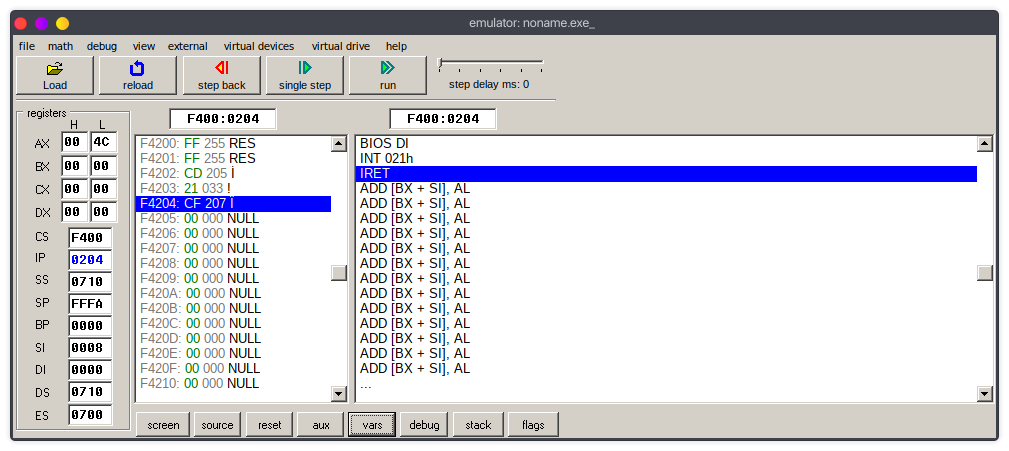
\includegraphics[width=0.90\textwidth]{img/p7/ss1.png}
	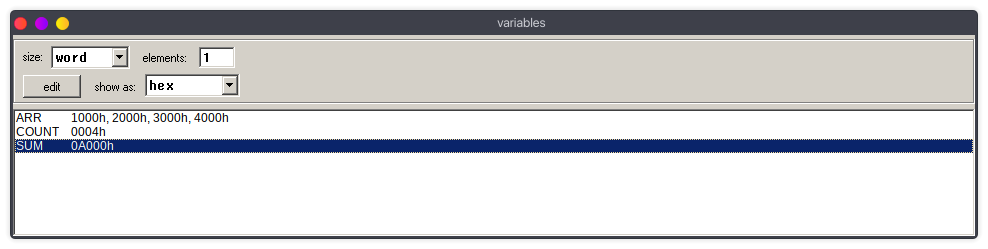
\includegraphics[width=0.90\textwidth]{img/p7/ss2.png}
\end{center}

\subsection{Result}
The sum of an 32 bit array was found out in emu8086
\newpage

\section{Element wise sum}
\subsection{Aim}
To find the element wise of two arrays

\subsection{Code}
\begin{lstlisting}
DATA SEGMENT
  arr1 DW 1000H, 2000H, 3000H, 4000H
  arr2 DW 4000H, 3000H, 2000H, 1000H
  sum DW 4 DUP(?)
  count DW 4
DATA ENDS

CODE SEGMENT
ASSUME CS:CODE, DS:DATA
START:
  MOV AX, DATA
  MOV DS, AX
  MOV CX, count
  LEA SI, arr1
  LEA DI, arr2
  LEA BX, sum

SUMLOOP:
  MOV AX, [SI]
  ADD AX, [DI]
  MOV [BX], AX
  ADD SI, 2
  ADD DI, 2
  ADD BX, 2
  LOOP SUMLOOP

EXIT:
  MOV AX, 4CH
  INT 21H
CODE ENDS
END START
\end{lstlisting}

\subsection{Output}
\begin{center}
	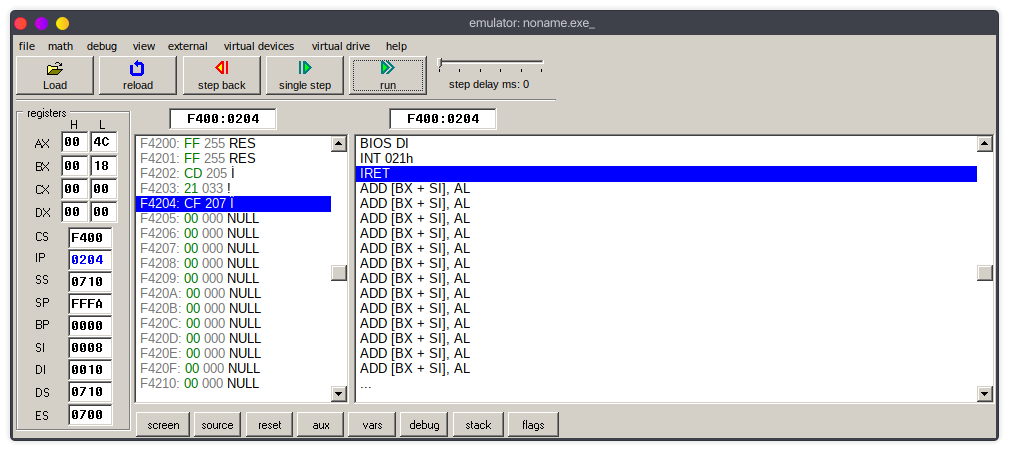
\includegraphics[width=0.90\textwidth]{img/p8/ss1.png}
	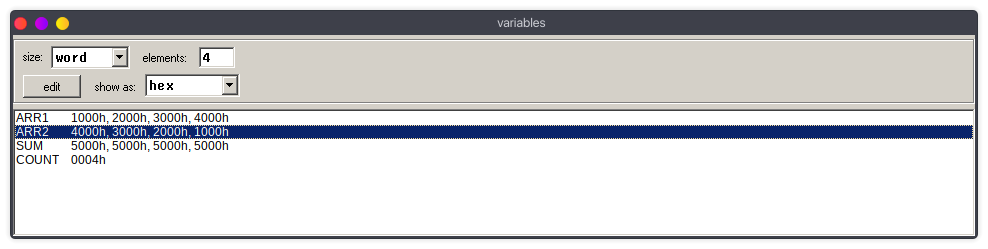
\includegraphics[width=0.90\textwidth]{img/p8/ss2.png}
\end{center}

\subsection{Result}
The element wise sum of two 32bit array was found in emu8086
\newpage

\section{Bubble sort}
\subsection{Aim}
To perform bubble sort on a list of numbers

\subsection{Code}
\begin{lstlisting}
DATA SEGMENT
  arr DW 1000H, 3000H, 4000H, 2000H
  count DW 4
DATA ENDS

CODE SEGMENT
ASSUME CS:CODE, DS:DATA
START:
  MOV AX, DATA
  MOV DS, AX
  XOR CX, CX
  XOR BX, BX

LOOP1:
  CMP CX, count
  JE EXIT
  XOR BX, BX
  LEA SI, arr
LOOP2:
  MOV AX, count
  SUB AX, CX
  SUB AX, 1
  CMP BX, AX
  JGE INCRLOOP1
  MOV AX, [SI]
  CMP AX, [SI+2]
  JL INCRLOOP2
  MOV AX, [SI]
  MOV DX, [SI+2]
  MOV [SI], DX
  MOV [SI+2], AX
INCRLOOP2:
  INC BX
  ADD SI, 2
  JMP LOOP2
INCRLOOP1:
  INC CX
  JMP LOOP1

EXIT:
  MOV AX, 4CH
  INT 21H
CODE ENDS
END START
\end{lstlisting}

\subsection{Output}
\begin{center}
	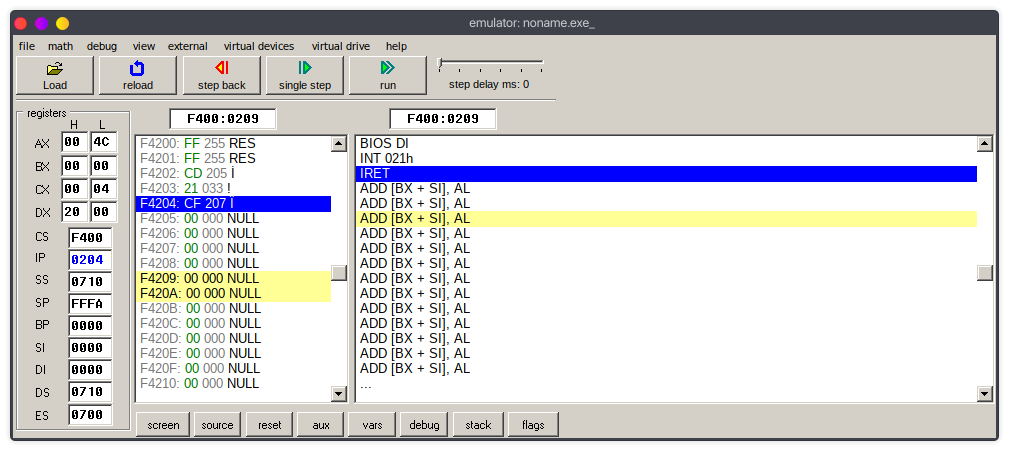
\includegraphics[width=0.90\textwidth]{img/p9/ss1.png}
	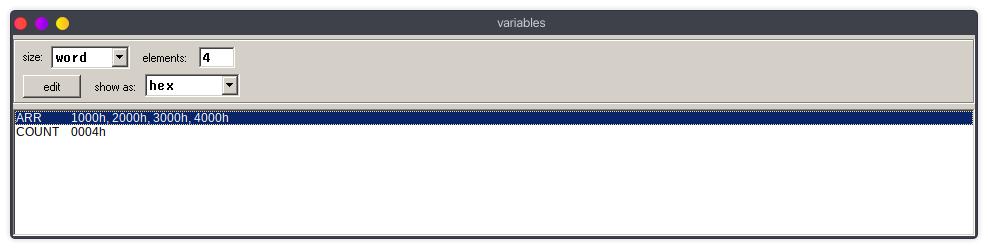
\includegraphics[width=0.90\textwidth]{img/p9/ss2.png}
\end{center}

\subsection{Result}
A 32bit array was sorted using bubble sort algorithm in emu8086
\newpage

\section{Largest element of array}
\subsection{Aim}
To find the largest element in the array

\subsection{Code}
\begin{lstlisting}
DATA SEGMENT
  arr DW 1000H, 3000H, 4000H, 2000H
  count DW 4
  largest DW ?
DATA ENDS

CODE SEGMENT
ASSUME CS:CODE, DS:DATA
START:
  MOV AX, DATA
  MOV DS, AX
  MOV CX, count
  LEA SI, arr
  XOR AX, AX

LARGELOOP:
  CMP AX, [SI]
  JGE INCRLOOP
  MOV AX, [SI]
INCRLOOP:
  ADD SI, 2
  LOOP LARGELOOP

EXIT:
  MOV largest, AX
  MOV AX, 4CH
  INT 21H
CODE ENDS
END START
\end{lstlisting}

\subsection{Output}
\begin{center}
	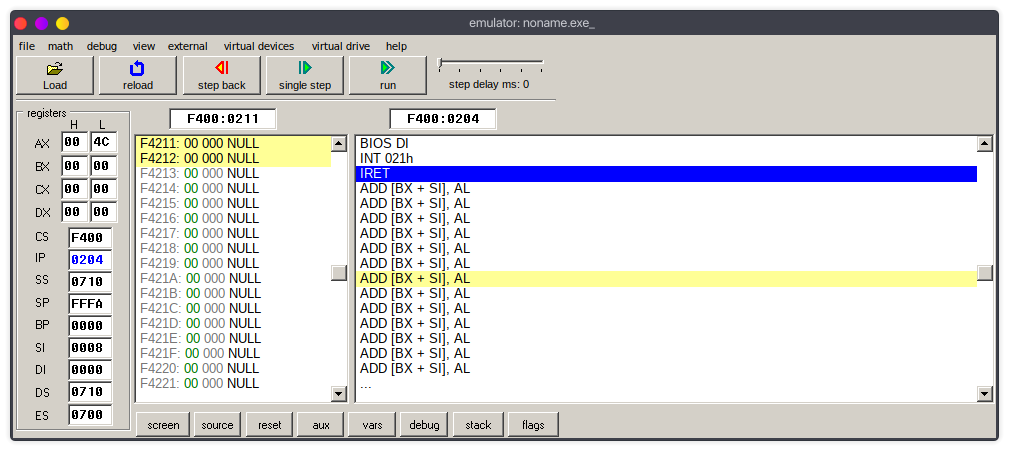
\includegraphics[width=0.90\textwidth]{img/p10/ss1.png}
	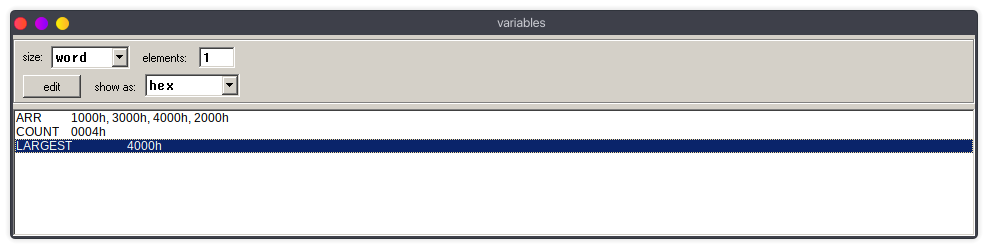
\includegraphics[width=0.90\textwidth]{img/p10/ss2.png}
\end{center}

\subsection{Result}
A largest element in an array was found out in emu8086
\newpage

\section{Linear Search}
\subsection{Aim}
To perform linear search on an array of numbers

\subsection{Code}
\begin{lstlisting}
DATA SEGMENT
  arr DW 1000H, 3000H, 4000H, 2000H
  count DW 4
  query DW 3001H
  msg1 DB "Found$"
  msg1len DW $-msg1
  msg2 DB "Not found$"
  msg2len DW $-msg2
DATA ENDS

CODE SEGMENT
ASSUME CS:CODE, DS:DATA
START:
  MOV AX, DATA
  MOV DS, AX
  MOV CX, count
  LEA SI, arr
  XOR AX, AX

SEARCHLOOP:
  MOV AX, query
  CMP AX, [SI]
  JE FOUND
INCRLOOP:
  ADD SI, 2
  LOOP SEARCHLOOP
  JMP NOTFOUND

FOUND:
  LEA DX, msg1
  MOV AH, 09H
  INT 21H
  JMP EXIT

NOTFOUND:
  LEA DX, msg2
  MOV AH, 09H
  INT 21H
  JMP EXIT  

EXIT:
  MOV AH, 4CH
  INT 21H
CODE ENDS
END START
\end{lstlisting}

\subsection{Output}
\begin{center}
	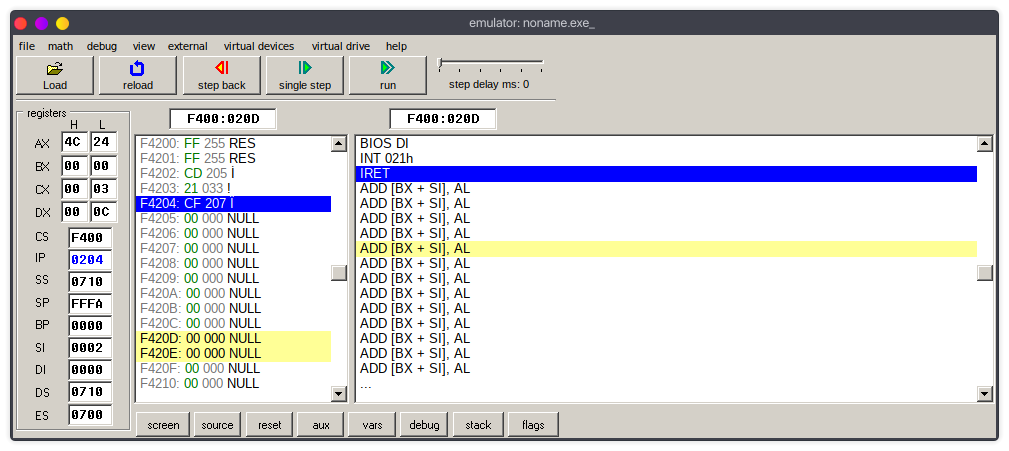
\includegraphics[width=0.90\textwidth]{img/p11/ss1.png}
	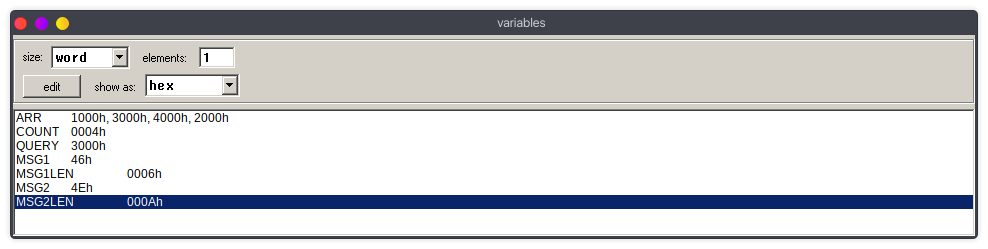
\includegraphics[width=0.90\textwidth]{img/p11/ss2.png}
	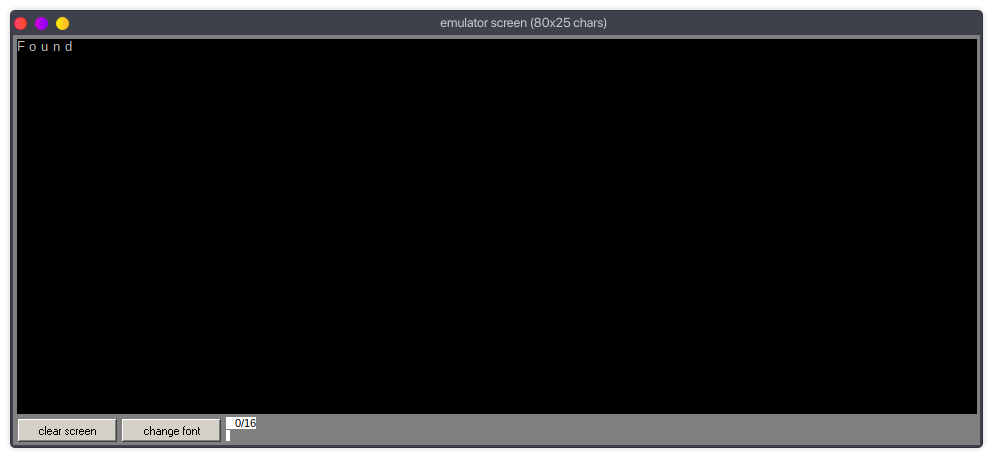
\includegraphics[width=0.90\textwidth]{img/p11/ss3.png}\\
  Output for 3000H\\
  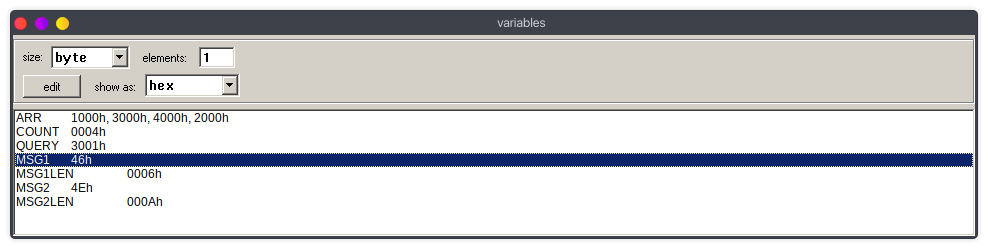
\includegraphics[width=0.90\textwidth]{img/p11/ss4.png}
	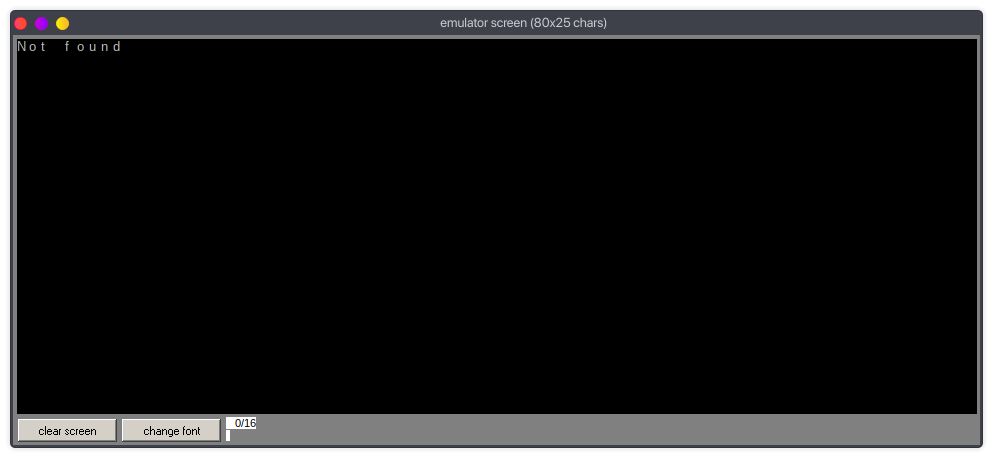
\includegraphics[width=0.90\textwidth]{img/p11/ss5.png}\\
  Output for 3001H
\end{center}

\subsection{Result}
Linear search was performed in an array in emu8086
\newpage

\section{Binary to BCD Conversion}
\subsection{Aim}
To convert a binary number to BCD

\subsection{Code}
\begin{lstlisting}
DATA SEGMENT
  bin EQU 1000b
  result DW ?
DATA ENDS

CODE SEGMENT
ASSUME CS:CODE, DS:DATA
START:
  MOV AX, DATA
  MOV DS, AX
  MOV BX, bin
  XOR AX, AX
  XOR CX, CX

CONVLOOP:
  CMP BX, 0
  JE EXIT
  DEC BX
  MOV AL, CL
  ADD AL, 01H
  DAA
  MOV CL, AL
  MOV AL, CH
  ADC AL, 00H
  DAA
  MOV CH, AL
  JMP CONVLOOP

EXIT:
  MOV result, CX
  MOV AX, 4CH
  INT 21H
CODE ENDS
END START
\end{lstlisting}

\subsection{Output}
\begin{center}
	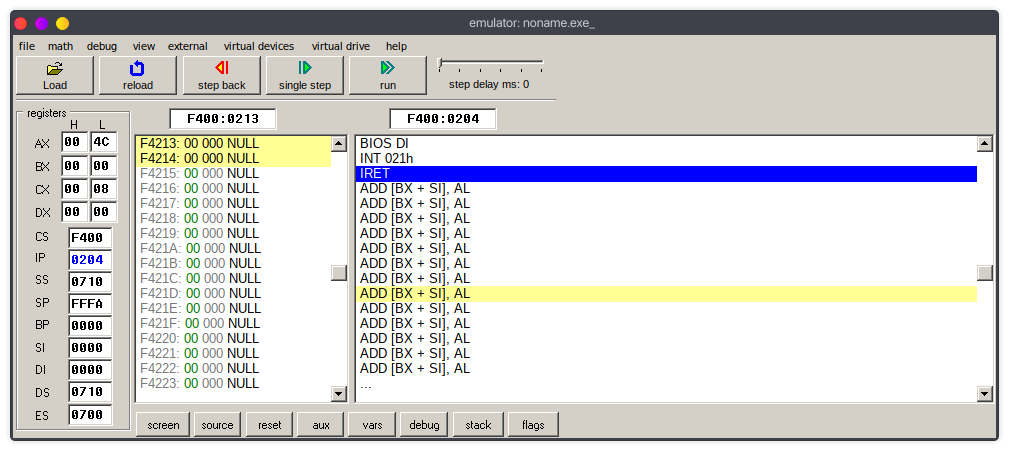
\includegraphics[width=0.90\textwidth]{img/p12/ss1.png}
	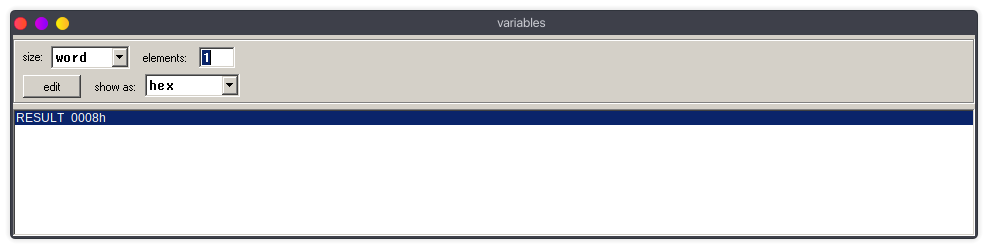
\includegraphics[width=0.90\textwidth]{img/p12/ss2.png}
\end{center}

\subsection{Result}
A binary number was converted to BCD in emu8086
\end{document}